\subsection{Introduction}\label{section:introduction}


Neuronal activity, usually measured through electroencephalography (EEG), is related to haemodynamical activity, measured through functional magnetic resonance imaging (fMRI). The first captures the dynamics of the electrical field, whose source is located from the firing neurons' action potentials. In its turn, the second measures the blood supply dynamics. These two while being studied simultaneously \cite{shibasaki2008human,yu2016building,he2018spatialtemporaldo,rojas2018study,brechet2019capturing,daly2019electroencephalography,cury2020sparse,abreu2021eeg} differ in many aspects such as: temporal and spatial resolution, brain functions captured, recording and hardware cost. Recently we have seen several studies that use deep neural network models \cite{goodfellow2016deep} to learn a mapping from EEG data to and from fMRI data \cite{liu2019convolutional, calhas2022eeg}. These are a type of generative model \cite{murphy2012machine}, that sample/synthesize instances from a different data source (instead of a distribution). Such a model could allow health care cost reductions and discoveries of new neuroscience insights on the relationship between these two modalities. Indeed, pathologies that require MRI scans diagnostics benefit from a lower cost EEG assessment, since availability of MRI hardware is very scarce \cite{ogbole2018survey}. As Python \cite{van1995python} becomes a hub for scientific development \cite{harris2020array,virtanen2020scipy,abadi2016tensorflow} we find the need to provide open source software that provides solutions for \textit{EEG to fMRI synthesis}, urgent, in order for third party scientific contributions coming from other laboratories to coexist and health care software integration to develop for diagnostic settings. To that end, we provide a description of the open source software \href{https://pypi.org/project/eeg-to-fmri/}{EEG-to-fMRI}, which originated from an academic scientific project funded by Funda\c{c}\~ao para a Ci\^encia e Tecnologia, and make publicly available a github \href{https://github.com/eeg-to-fmri/eeg-to-fmri}{repository}.

\subsection{Methods}\label{section:methods}

The mapping function provided in this software is the one proposed by \cite{calhas2022eeg}. It consists on transforming the EEG from a channel by time representation to a channel by time-frequency one, achieved using the short time Fourier transform \cite{allen1977short} by means of the fast Fourier transform (\href{https://docs.scipy.org/doc/scipy/reference/generated/scipy.fft.fft.html}{scipy.fft.fft}) available in the SciPy package. The latter corresponds to the second step of the diagram illustrated in \ref{fig:pipeline}. In the second step, this representation is then forward through a deep neural network (implemented as a \href{https://www.tensorflow.org/api_docs/python/tf/keras/Model}{tf.keras.Model}), with contributions ranging from Resnet blocks \cite{he2016deep}, an automated machine learning framework \cite{calhas2022automatic} and Fourier features \cite{tancik2020fourier}. Ultimately, this enables the prediction of an fMRI volume associated with a $26$ second segment of an EEG recording. 

\begin{figure*}[t]
    \centering
    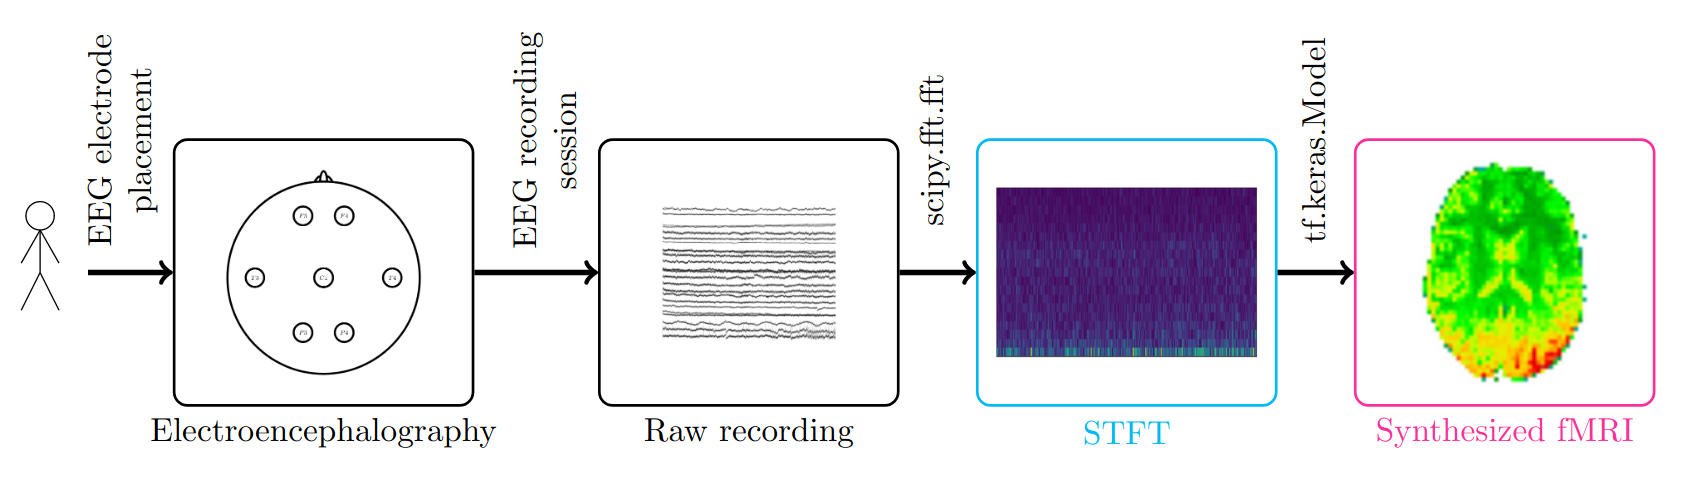
\includegraphics[width=0.8\textwidth]{figures/diagram.png}
    \caption{The pipeline of the EEG to fMRI synthesis project consists of processing EEG recordings, that are sourced from a human subject that goes through an EEG recording sesssion, then processing the channel by time signal and taking the short time Fourier transform. The latter, gives us the time frequency representation of the EEG signal. The novelty of this software is that it provides a model that given as input the EEG signal it predicts the corresponding fMRI volume associated with that segment. A video demonstration of the whole pipeline is available on \href{https://youtu.be/47uJbI0hU_I}{Youtube}.}
    \label{fig:pipeline}
\end{figure*}

\subsection{Description}\label{section:description}

The dependencies of each component are described in an \href{https://github.com/eeg-to-fmri/eeg-to-fmri/blob/main/project_UML.pdf}{UML diagram}. Overall to install the package, the user is required to install the following dependencies: \textit{tensorflow 2.9.0}, \textit{matplotlib 3.5.3}, \textit{mne 0.23.4}, \textit{nilearn 0.7.0}, \textit{tensorflow probability 0.12.2}, \textit{tensorflow determinism 0.3.0}, and \textit{tensorflow addons 0.19.0}. As seen there is a high dependency in tensorflow related packages. This is due to the whole system provided being built in tensorflow, a library that enables automatic differentiation and is widely used for deep learning model development.

\subsubsection{Package modules}\label{section:modules}

This package, as it is provided, has eight main modules:
\begin{itemize}
    \item \textit{models}: here you will find the code that implements the models for synthesis and classification. The synthesis models are located in the \textit{synthesizers.py}, where the class \textit{EEG\_to\_fMRI} is implemented. This class defines a \textit{tf.keras.Model}, composed of two encoders, one for the EEG and another for the fMRI. Additionally, there is a decoder that maps the latent EEG representation, that is the output of the EEG encoder, to the estimate of the fMRI volume associated. The fMRI encoder is defined in the \textit{fmri\_ae.py} file. The task would not be complete without the extrapolation of the synthesis model to a classification task. To that end, two linear classifiers are provided, the \textit{ViewLatentContrastiveClassifier} and the \textit{ViewLatentLikelihoodClassifier}, corresponding to a contrastive latent loss and a cross entropy error driven classification, respectively. The extrapolation is simply made by taking the output of the neural flow that comes from the EEG, that is the EEG encoder and the decoder.
    \item \textit{layers}: this module contains the layers which compose the synthesizer models. Five main types of layers should be considered. First, the \textit{TopographicalAttention} computes a self attention mechanism in the channels dimension of the EEG \cite{calhas2022eeg}, this allows the representation to be correctly processed by the convolutional blocks. Second, the \textit{ResnetBlock} \cite{he2016deep} is a layer corresponds to the implementation of a residual block that is composed of convolutional layers. This block allows efficient gradient propagation by tackling the vanishing gradient phenomena. Third, the \textit{FourierFeatures} is a layer that projects sinusoid functions, namely \textit{cosines}, of different shifts and biases, to build a latent spectral basis for the prediction of the fMRI volume. Fourth, the \textit{DenseVariational} is an implementation of the \textit{tf.keras.layers.Dense} for two dimensional inputs, whose weights are drawn from gaussian distributions. Last, but not least, we provide the \textit{DCT} based layers, which implement the discrete cosine transform \cite{ahmed1974discrete}. These layers are useful for alternative ways of decoding the latent representation of the EEG to produce the desired fMRI volume;
    \item \textit{regularizers}: here the implementation of different regularizers for the synthesizer model is provided. Most importantly in the \textit{activity\_regularizers.py} file is found the \textit{OrganizeChannels} implementation which can be added in the \textit{TopographicalAttention} layer, so that the layer does not surpress any channel;
    \item \textit{learning}: here are implemented the routines for the optimization of the models, namely the \textit{losses} and the \textit{train} procedures. The \textit{train.py} is a generalizable training routine that fits any type of \textit{tf.keras.Model} instance. Following, the \textit{losses.py} contain a set of losses that are implemented to train the models provided in the \textit{models} module. Most importantly, here you will find the \textit{mae\_cosine} for the deterministic versions of the \textit{EEG\_to\_fMRI} model, the \textit{LaplacianLoss} for variational versions, and the \textit{ContrastiveClassificationLoss} which serves as the cost function for the \textit{ViewLatentContrastiveClassifier}; 
    \item \textit{explainability}: this module contains explainability mehtods that were employed for the models developed. The implementation for the layer wise relevance propagation \cite{bach2015pixel} can be found in \textit{lrp.py}. In particular, since this type of algorithm is not model agnostic, we have the implementation for all the permutations' of operations that the \textit{EEG\_to\_fMRI} model can have;
    \item \textit{data}: this is maybe the most important module for researchers wanting to try out their collected data with this software. Here all of the functions, that read data and manipulate it as such to allow the efficient training, are implemented. Starting with the \textit{eeg\_utils.py}, where the \textit{get\_eeg\_instance\_<DS>} function is implemented for a limited set of datasets that participated in the experiments of the associated studies. The <DS> stands for the identifier of the dataset. Currently there are a set of functions implemented for publicly available datasets. Please check the description of the code in the github repository for more details. In the \textit{fmri\_utils.py} file one finds functions of the form \textit{get\_individuals\_paths\_<DS>}, that have the exact same function as the functions to read EEG recordings, but in this case they read nifti file format. These type of files are the standard format for fMRI recordings. Finally, the \textit{data\_utils.py} and \textit{preprocessed\_data.py} are responsible for concatenating the EEG and fMRI instance pairs, with all the alignments and event synchronization events taken into account, as well as the processing to build \textit{tf.data.Dataset} classes.
    \item \textit{metrics}: in this module are implemented the metrics usually used to evaluate synthesis of tgenerated images, such as the root mean squared error, mean absolute error, structural similarity index measure \cite{wang2004image}, among others; 
    \item \textit{utils}: Last but not least, is the utilities module, which provides the user with print functions, configuration of the tensorflow environments and several visualizations that were used in the original studies that developed the package.
\end{itemize}

\begin{figure*}[t]
    \centering
    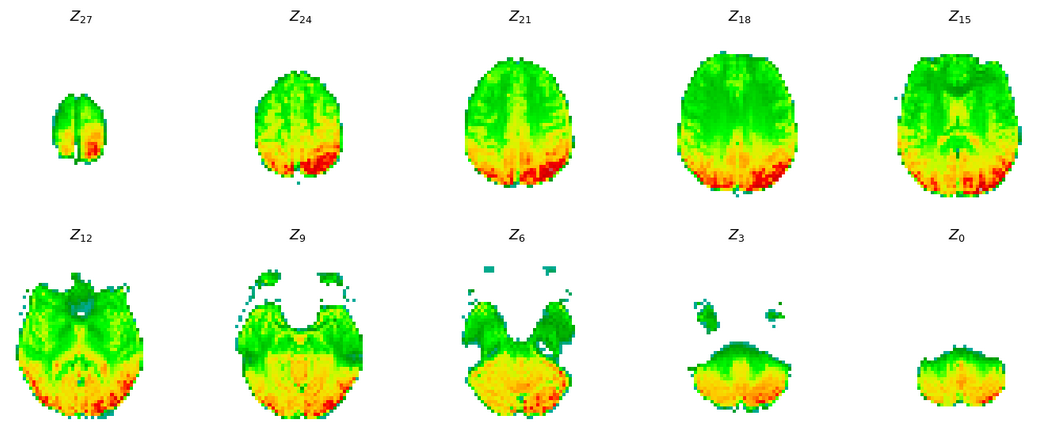
\includegraphics[width=\textwidth]{figures/sythesized.png}
    \caption{The synthesized signal of fMRI. This is the output visualization when running the code for the classification notebook.}
    \label{fig:synthesized}
\end{figure*}

\subsubsection{New data integration}\label{section:new_data}

In order to use the software provided for new data, we recommend that the dataset is structured as shown in Figure \ref{fig:structure}.
\begin{figure}[ht]
    \centering
    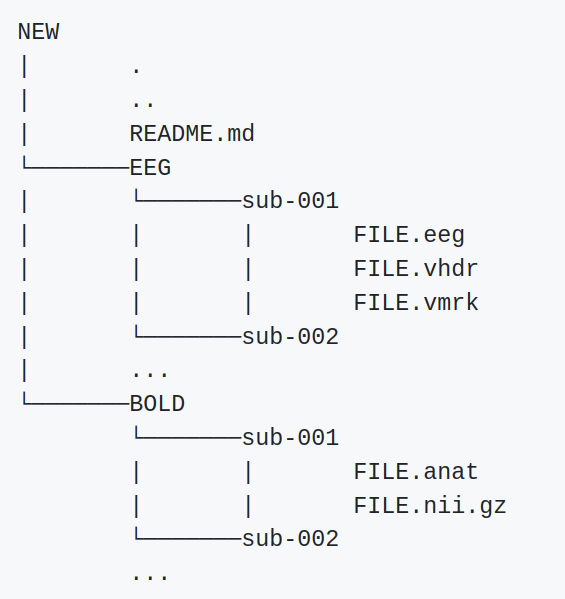
\includegraphics[width=0.45\textwidth]{figures/structure.png}
    \caption{Recommended structure of the dataset directory.}
    \label{fig:structure}
\end{figure}
If the data is provided as illustrated then the user only has to name the directory of the data as \textit{01}. This should suffice for the correct loading of the data. Any type of issue that is encountered for this package should be published as an issue in the official github repository.

\subsubsection{Building an EEG to fMRI model}\label{section:build_model}

For the user to build an EEG to fMRI model, they have to first import the correct library module and \textit{tensorflow}.
\begin{Verbatim}[commandchars=\\\{\},fontsize=\footnotesize]
    \PY{k}{from} tensorflow \PY{k}{as} tf
    \PY{k}{from} eeg_to_fmri.models.synthesizers 
            \PY{k}{import} EEG_to_fMRI
    \PY{k}{from} eeg_to_fmri.models.synthesizers 
            \PY{k}{import} parameters
    \PY{k}{from} eeg_to_fmri.models.synthesizers
            \PY{k}{import} na_specification_eeg
    \PY{k}{from} eeg_to_fmri.models.fmri_ae 
            \PY{k}{import} na_specification_fmri
\end{Verbatim}
Let us define the size of the EEG representation $\vec{x} \in \mathbb{R}^{64\times 134\times 10 \times 1}$, the fMRI representation  $\vec{y} \in \mathbb{R}^{64\times 64\times 30\times 1}$, and the latent representation, for both the EEG and fMRI, that is $\vec{z}_x,\vec{z}_y \in \mathbb{R}^{7\times 7\times 7}$.
\begin{Verbatim}[commandchars=\\\{\},fontsize=\footnotesize]
    \PY{n}{fmri_dim}\PY{o}{=}\PY{n}{(64,134,10,1)}
    \PY{n}{fmri_dim}\PY{o}{=}\PY{n}{(64,64,30,1)}
    \PY{n}{latent_dim}\PY{o}{=}\PY{n}{(7,7,7)}
\end{Verbatim}
Then, we have to define the parameters for the model, these are provided as a variable in the \textit{synthesizers.py}.
\begin{Verbatim}[commandchars=\\\{\},fontsize=\footnotesize]
    \PY{n}{learning_rate},\PY{n}{weight_decay},\PY{n}{kernel_size},
    \PY{n}{stride_size},\PY{n}{batch_size},\PY{n}{latent_dimension},
    \PY{n}{n_channels},\PY{n}{max_pool},\PY{n}{batch_norm},
    \PY{n}{skip_connections},\PY{n}{dropout},
    \PY{n}{n_stacks},\PY{n}{outfilter},\PY{n}{local}\PY{o}{=}\PY{n}{parameters}
\end{Verbatim}
Some of these parameters will also be used to define the fMRI encoder. Since the fMRI encoder is a different class, we need to define the initialization parameters.
\begin{Verbatim}[commandchars=\\\{\},fontsize=\footnotesize]
    \PY{n}{fmri_parameters}\PY{o}{=}(\PY{n}{parameters}, \PY{n}{latent_dim}, 
        \PY{n}{fmri_dim}, \PY{n}{kernel_size}, \PY{n}{stride_size}, 
        \PY{n}{n_channels}, \PY{n}{max_pool}, \PY{n}{batch_norm}, 
        \PY{n}{weight_decay}, \PY{n}{skip_connections}, 
        \PY{n}{n_stacks}, \PY{k}{True}, \PY{n}{False}, 
        \PY{n}{outfilter}, \PY{k}{dropout}, \PY{k}{None}, 
        \PY{k}{False}, \PY{n}{na_specification_fmri})
\end{Verbatim}
Next, we have all of the parameters necessary to build a simple deterministic version of the EEG to fMRI model.
\begin{Verbatim}[commandchars=\\\{\},fontsize=\footnotesize]
    \PY{k}{with} tf.device(\PY{s}{'/CPU:0'}):
        \PY{n}{model} \PY{o}{=} EEG_to_fMRI(\PY{n}{latent_dim}, \PY{n}{eeg_dim}, 
            \PY{n}{na_specification_eeg}, \PY{n}{n_channels}, 
            \PY{n}{weight_decay}\PY{o}{=}\PY{n}{weight_decay}, 
            \PY{n}{skip_connections}\PY{o}{=}\PY{k}{True}, \PY{n}{batch_norm}\PY{o}{=}\PY{k}{True}, 
            \PY{n}{fourier_features}\PY{o}{=}\PY{k}{True}, 
            \PY{n}{random_fourier}\PY{o}{=}\PY{k}{True}, 
            \PY{n}{topographical_attention}\PY{o}{=}\PY{k}{True}, 
            \PY{n}{conditional_attention_style}\PY{o}{=}\PY{k}{True},
            \PY{n}{conditional_attention_style_prior}\PY{o}{=}\PY{k}{False}, 
            \PY{n}{local}\PY{o}{=}\PY{k}{True}, \PY{n}{seed}\PY{o}{=}\PY{k}{None}, 
            \PY{n}{fmri_args} \PY{o}{=} \PY{n}{fmri_parameters})
\end{Verbatim}
The model is built once it is specified the input dimension, this is done through the \textit{tf.keras.Layer\#build}. This will initialize all of the weights of the network.
\begin{Verbatim}[commandchars=\\\{\},fontsize=\footnotesize]
    \PY{n}{model.build((None,)+eeg_dim, (None,)+fmri_dim)}
\end{Verbatim}

\subsubsection{Cost function and optimization}

Regarding the cost function, which is provided in the \textit{learning} module at the \textit{losses.py} file, we can specify different metrics that are provided. Take, for instance, the example of using an approximation of the mean absolute error at the output for the fMRI volume prediction $\hat{\vec{y}}$, and approximation of the latent representations of the fMRI as proposed by \cite{calhas2022eeg}. This is reduced to the mathematical formula
\begin{equation}\label{equation:loss}
    \mathcal{L}(\vec{x}, \vec{y}, \vec{z}_x, \vec{z}_y) = ||\vec{y} - \hat{\vec{y}}||_1^1 + 1 - \frac{\vec{z}_x \cdot \vec{z}_y}{||\vec{z}_x||_2^2 ||\vec{z}_y||_2^2}.
\end{equation}
In terms of code, this is already implemented and can be loaded directly.
\begin{Verbatim}[commandchars=\\\{\},fontsize=\footnotesize]
    \PY{k}{from} eeg_to_fmri.learning \PY{k}{import} losses
    \PY{n}{loss_fn}=\PY{n}{losses.mae_cosine}
\end{Verbatim}
The optimizer is already provided in the \textit{tensorflow} library and its corresponding learning rate is given in the parameters variable.
\begin{Verbatim}[commandchars=\\\{\},fontsize=\footnotesize]
    \PY{n}{optimizer}=
            \PY{n}{tf.keras.optimizers.Adam(learning_rate)}
\end{Verbatim}
Training the model requires an input, the EEG $\vec{x}$, and an output, the fMRI $\vec{y}$. The architecture processes both the EEG and fMRI, producing the latent representation for both. Proceeding the latent EEG representation, $\vec{z}_x$, is fed to the decoder which estimates the fMRI $\hat{\vec{y}}$.
\begin{Verbatim}[commandchars=\\\{\},fontsize=\footnotesize]
    \PY{k}{def} apply_gradient(model, optimizer, loss_fn, 
        x, y, return_logits=\PY{k}{False}, call_fn=None):
        \PY{k}{with} tf.GradientTape(persistent=\PY{k}{True}) \PY{k}{as}
                                            tape:
            logits=model(*x, training=\PY{k}{True})
            regularization=0.
            \PY{k}{if}(len(model.losses)):
                regularization=
                    tf.math.add_n(model.losses)
            loss=loss_fn(y, logits)+regularization
        gradients=tape.gradient(loss, 
                model.trainable_variables)
        optimizer.apply_gradients(zip(gradients,
            model.trainable_variables))
        \PY{k}{return} tf.reduce_mean(loss)
\end{Verbatim}
The training routine functions are found in the \textit{learning} module. The function \textit{apply\_gradient} computes the forward and backward pass of the neural network. Note that the input of the \textit{EEG\_to\_fMRI} model is composed of two tensors, which is the reason why one unrolls the tuple as \textit{*x}. One the loss is computed, which computes both the estimation of the fMRI according to the mean absolute error (MAE) and the cosine distance between the latent representations, the regularization terms are also added to the loss. Note that, these regularization terms refer to weight decay and other activity regularizers that may or may not participate in the model. The loss function often used for the synthesis task, the one used in \cite{calhas2022eeg}, is the MAE and the cosine distance. This loss function is defined in the \textit{learning} module, found at the \textit{losses.py} file. This loss receives a \textit{tf.Tensor} object, \textit{y\_true}, and a list of \textit{tf.Tensor}. The list of tensors contains the outputs of the neural network that should be approximated. The first element of the list is the estimated fMRI volume and the second and third items are the latent EEG and fMRI representations, respectively.
\begin{Verbatim}[commandchars=\\\{\},fontsize=\footnotesize]
    \PY{k}{def} mae_cosine(y_true, y_pred):
        \PY{k}{return} tf.reduce_mean(
            tf.math.abs(y_pred[0] - y_true), 
            axis=(1,2,3)) +
            cosine(y_pred[1], y_pred[2])
\end{Verbatim}
At test time, the \textit{EEG\_to\_fMRI} model can discard the fMRI input. To that end, only the decoder attribute is called, which is composed of the EEG encoder and the decoder. 
\begin{Verbatim}[commandchars=\\\{\},fontsize=\footnotesize]
    \PY{k}{def} call(self, x1, x2):
        \PY{k}{if}(self.training):
            \PY{k}{return} [self.decoder(x1), 
                self.eeg_encoder(x1), 
                self.fmri_encoder(x2)]

        \PY{k}{return} self.decoder(x1)
\end{Verbatim}
Note that, the \textit{pretrained\_EEG\_to\_fMRI} class processes a pretrained model of the type \textit{EEG\_to\_fMRI} and builds a new model that only processes EEG and outputs an fMRI prediction given the representation learned. This class is built to be then appended with a classifier, that can be either a \textit{ViewLatentContrastiveClassifier} or a \textit{ViewLatentLikelihoodClassifier}.

\subsection{Examples}\label{section:examples}

In this section, we walk through the examples given in jupyter notebooks. 

\subsubsection{Synthesis}\label{section:synthesis}


We provide a compressed version of the dataset of \cite{dataset2014noddi}. Users can directly execute the code and have both the python package, as well as the dataset, setup in a google colab environment. The flow of execution has been already described. In the end a synthesized fMRI is shown, as illustrated in Figure \ref{fig:synthesized}. This image is built using the \textit{viz\_utils.py}. The user can find metrics for synthesis evaluation in \textit{eeg\_to\_fmri.metrics.quantitative\_metrics}. We report results from the \cite{calhas2022eeg} study on the NODDI dataset \cite{dataset2014noddi}. An example with a reduced dataset is available in \href{https://github.com/eeg-to-fmri/eeg-to-fmri/blob/main/examples/synthesis.ipynb}{synthesis notebook}. The best model, which used the configuration of the \textit{eeg\_to\_fmri.models.synthesizers.EEG\_to\_fMRI} achieved $0.3972$  RMSE and $0.4613$ SSIM. This constitutes the state-of-the-art for this task and provides a view that can be applied in EEG only datasets for classification task (as shown in the \href{https://github.com/eeg-to-fmri/eeg-to-fmri/blob/main/examples/classification_contrastive.ipynb}{classification notebook} example).

\subsubsection{Classification}\label{section:classification}

\begin{figure*}[t]
    \centering
    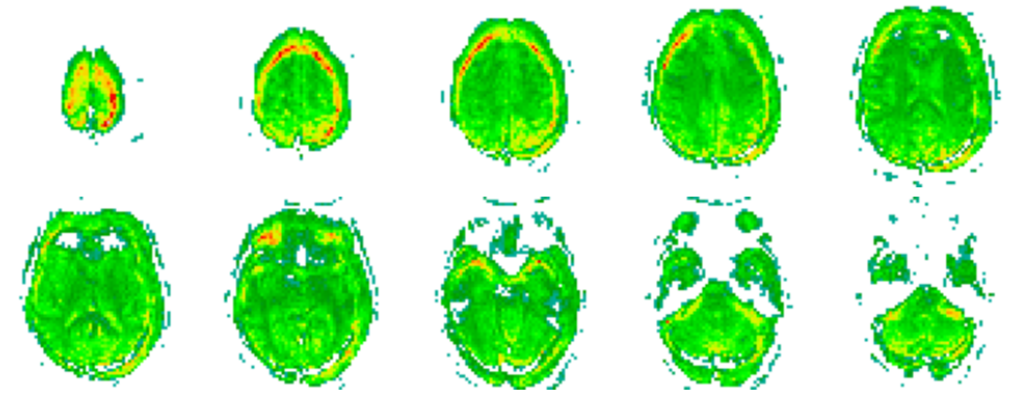
\includegraphics[width=\textwidth]{figures/discriminative.png}
    \caption{Output of the predicted fMRI when given an EEG representation. Note that, due to the EEG encoder being optimized towards classifying the data according to the groups of individuals defined, e.g. schizophrenic and healthy controls, the decoder (that has the parameters frozen) is given a slighthly altered representation. This change is seen in the produced fMRI.}
    \label{fig:discriminative}
\end{figure*}
We also provide a compressed version of the dataset of \cite{dataset2022fribourg}. This example is based on a public available dataset that contains individuals diagnosed with schizophrenia and healthy controls. The whole goal of the project is to be applied in an health care setting and to this end we employ an end to end software solution. The whole software package is able to synthesize fMRI and adapt to a classification setting, that given EEG recordings it outputs a set of probabilities for each group of people considered in the dataset.

%\begin{figure*}[t]
%    \centering
%    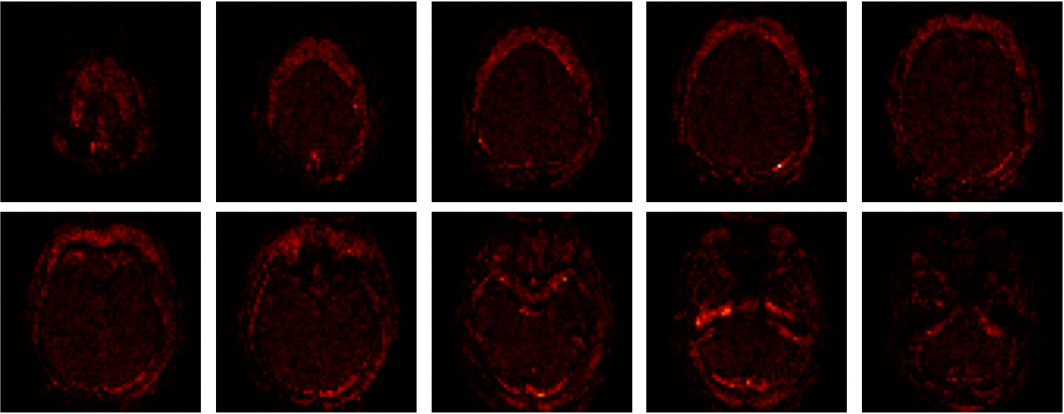
\includegraphics[width=\textwidth]{figures/scz_explanations.png}
%    \caption{}
%    \label{fig:scz_explanations}
%\end{figure*}

%\begin{figure*}[t]
%    \centering
%    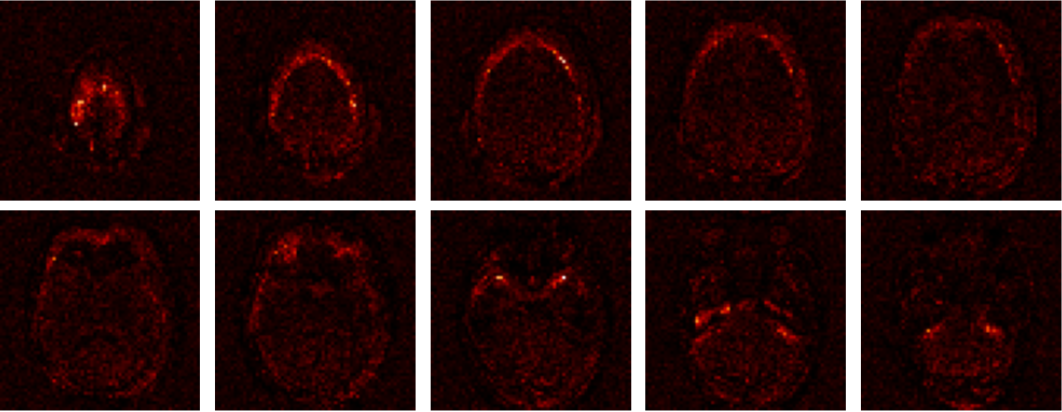
\includegraphics[width=\textwidth]{figures/hc_explanations.png}
%    \caption{}
%    \label{fig:hc_explanations}
%\end{figure*}

\subsection{Collaboration}\label{section:collabs}

Ultimately, the goal of this package is to collect, in one package, methods for EEG to fMRI synthesis. We would welcome contributions from authors of related work such as \cite{liu2019convolutional}. In the future, we plan to add a module or example folder with implementations of these approaches, so that other research groups can easily access them and reproduce key results. 

On a higher level, this software is encouraged for testing its applicability in health care settings. The impact, that such mappings from EEG to fMRI, would have on society is enormous, given that the diagnostic is faithful. Take for instance the example of the MRI machine density across the African continent. In the worst case scenario, Nigeria has a density of 0.33 MRI machines per million people, according to \cite{ogbole2018survey}. To let that sink in, imagine having to wait in a line of 3 million people to get a diagnostic exam. This type of waiting bottleneck impacts greatly the development of diseases for the worse. Countries in such conditions would greatly benefit from contributions that further advance this scientific field. Even fortunate countries, whose economy thrives, that are able to provide their populations with a good ratio of MRI machines, they still have small portions of the population who live in remote areas. These people find it hard to get quality health care, without having to travel significant distances.  

\subsection{Conclusion}\label{section:conclusion}

This is the first package, to the best of our knowledge, that provides a machine learning oriented synthesis between functional neuroimaging modalities (EEG and fMRI). It is targeted to help the neuroscience community, in tasks such as modality augmentation, resolution enhancement, neuroimaging explainability techniques, among others. We hope to motivate researchers, scientists, and software developers to contribute to this package which we have been so passionate about throughout the last years.


 \subsection{Acknowledgments}\label{section:acknowledgments}

This work was supported by national funds through Funda\c{c}\~ao para a Ci\^encia e Tecnologia under the PhD Grant SFRH/BD/5762/2020 to David Calhas.
